% Author : Nicolas Moulin 

\documentclass[t,9pt,pdftexx,xcolor=dvipsnames]{beamer}
\usetheme{tb}
%\usepackage{ucs}
\usepackage[T1]{fontenc}
\usepackage[french]{babel}
\usepackage[utf8]{inputenc}
%\usepackage[utf8x]{inputenc}
\usepackage{textcomp}
\usepackage{graphicx}

%\setbeamertemplate{navigation symbols}[horizontal]
\usepackage{listingsutf8}
\usepackage{multicol}
\usepackage{animate}
\usepackage{multimedia}

\usepackage{listings}

 \lstset
{ 
  language=R,                     % the language of the code
  basicstyle=\normalsize\ttfamily, % the size of the fonts that are used for the code
  numbers=left,                   % where to put the line-numbers
  numberstyle=\tiny\color{Blue},  % the style that is used for the line-numbers
  stepnumber=1,                   % the step between two line-numbers. If it is 1, each line
                                  % will be numbered
  numbersep=5pt,                  % how far the line-numbers are from the code
  backgroundcolor=\color{white},  % choose the background color. You must add \usepackage{color}
  showspaces=false,               % show spaces adding particular underscores
  showstringspaces=false,         % underline spaces within strings
  showtabs=false,                 % show tabs within strings adding particular underscores
  frame=single,                   % adds a frame around the code
  rulecolor=\color{black},        % if not set, the frame-color may be changed on line-breaks within not-black text (e.g. commens (green here))
  tabsize=2,                      % sets default tabsize to 2 spaces
  captionpos=b,                   % sets the caption-position to bottom
  breaklines=true,                % sets automatic line breaking
%  breakatwhitespace=false,        % sets if automatic breaks should only happen at whitespace
  keywordstyle=\color{RoyalBlue},      % keyword style
  commentstyle=\color{ForestGreen},   % comment style
  stringstyle=\color{ForestGreen},      % string literal style
 extendedchars=true,
 literate={è}{{\`e}}1 {à}{{\'a}}1 {é}{{\'e}}1
} 



\graphicspath{{Figs/}}

\setbeamertemplate{caption}{\raggedright\insertcaption\par}

\title[Soutenance projet industriel]{Prévision de durées d'hospitalisation aux Hospices Civils de Lyon (HCL)\\}
\author[Grégoire MASSOT]{Grégoire MASSOT}

\date{21/01/2016}

\begin{document}

\inserttitlepage

\begin{frame}[c]
 \frametitle{Plan}
 % Plusieurs choix possibles (décommenter le choix sélectionné, commenter les autres):
 % Uniquement les sections principales : 
 \tableofcontents[hideallsubsections]
 % Sections et sous sections : 
 %\tableofcontents
\end{frame}
\AtBeginSection[]
  {
     \begin{frame}<beamer>
     \frametitle{Plan}
     \tableofcontents[currentsection]
     \end{frame}
  }
\section{Présentation du projet}

\begin{frame}[c]
\frametitle{Déroulement du projet}
 \begin{itemize}
 \item \textbf{Entreprise} : Hospices civils de Lyon
 \item \textbf{Tuteur entreprise} : Antoine DUCLOS - Médecin à Lyon
 \item \textbf{Tuteur école} : Thierry GARAIX
 \end{itemize}
\end{frame}

\begin{frame}[c]
\frametitle{Déroulement du projet}
 \begin {figure}[!ht]
 \begin{center}
 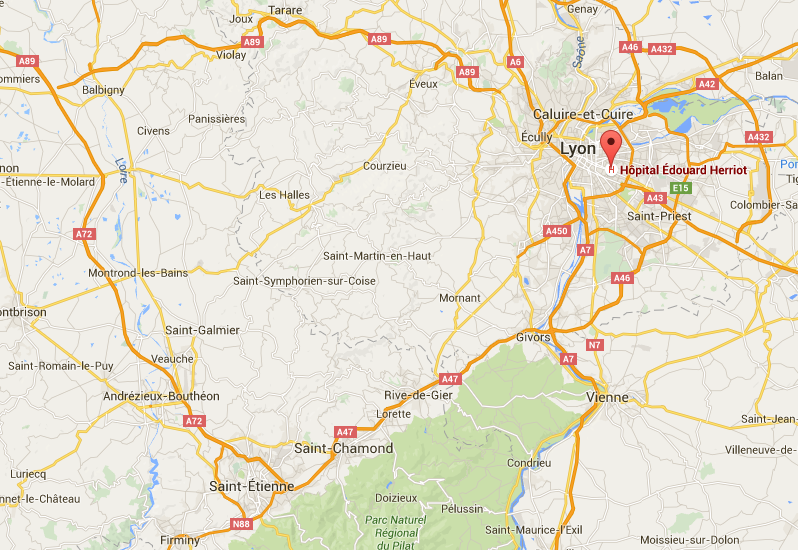
\includegraphics [width =8cm]{Map.PNG}
 \end{center}
 \end{figure}
 \begin{center}
  4 venues à Lyon : 20 Octobre, 6 Novembre, 11 Décembre, 15 Janvier.
 \end{center}
\end{frame}

\begin{frame}[c]
 \frametitle{Contexte du projet}
 Les HCL doivent optimiser la gestion de leurs ressources pour accueillir le plus de patients avec les ressources disponibles.
\end{frame}

\begin{frame}[c]
 \frametitle{Contexte du projet}
 Prévoir la durée d'hospitalisation des patients permet de maximiser l'occupation des lits
\end{frame}

\begin{frame}[c]
 \frametitle{Contexte du projet}
 Les HCL souhaitent utiliser leur base de données sur les patients précédents pour prédire les durées d'hospitalisation des nouveaux patients.
\end{frame}

\begin{frame}[c]
 \frametitle{Position du problème}
 \textbf{Objectif du PI} : déterminer la durée d'hospitalisation d'un patient à partir des données recueillies lors de son arrivée à l'hôpital et des statistiques sur les patients précédents.
\end{frame}

\begin{frame}[c]
\frametitle{Position du problème}
 \begin{figure}
 \caption{Schéma de la Base de données anonymisée des HCL}
 \begin{center}
 \begin{tabular}{|c|c|c|c|c|}
 \hline
 \textbf{Duree du séjour} & Âge du patient & Diagnostic principal & Service hospitalier & ...\\
 \hline
 \textbf{duree1} & age1 & dp1 & service1 & ... \\
 \hline
 \textbf{duree2} & age2 & dp2 & service2 & ... \\
 \hline
 \textbf{duree3} & age3 & dp3 & service3 & ... \\
 \hline
 \textbf{...} & ... & ...  & ... & ...\\
 \hline
 \end{tabular}
 \end{center}
 \end{figure}
\end{frame}

\section{Démarche}

\begin{frame}[c]
\frametitle{Démarche}
 Reprise du code R du challenge "Éolienne" de la majeure Data Science
 
 \begin {figure}[!ht]
 \begin{center}
 
\includegraphics [width =5cm]{Logo_Octo.png}
 \end{center}
 \end{figure}
\end{frame}

\begin{frame}[c]
\frametitle{Démarche}
 Inscription au challenge Walmart sur kaggle.com
 
 \begin {figure}[!ht]
 \begin{center}
 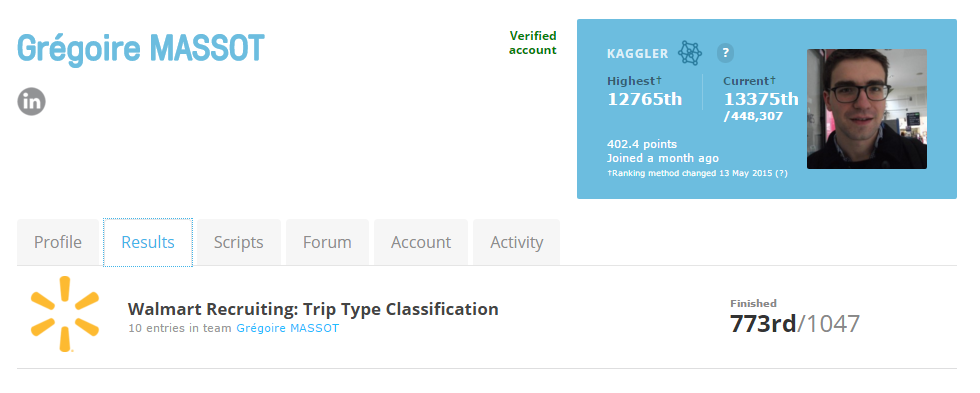
\includegraphics [width =10cm]{Profil_Kaggle.PNG}
 \end{center}
 \end{figure}
\end{frame}

\section{Code R}

\begin{frame}[c, fragile]
\frametitle{Code R - Chargement et sélection des données}
 \begin{lstlisting}
# Chargement de la BDD
donnees_hcl <- read.csv2(file = "base_ano.txt",header = TRUE, sep="\t")
# Sélection des séjours de durée supérieure ou égale à 1 jour
donnees_hcl <- donnees_hcl[donnees_hcl$duree >= 1,]
#Selection des prédicteurs effectivement disponibles lors de l'entrée du patient
donnees_hcl <- donnees_hcl[,-seq(8,57)]
donnees_hcl <- subset(donnees_hcl, select = -c(moissor))
donnees_hcl <- subset(donnees_hcl, select = -c(sortie))
donnees_hcl <- subset(donnees_hcl, select = -c(ID))

# Transformation du facteur "age" en variable continue
donnees_hcl$age <- as.character(donnees_hcl$age)
donnees_hcl$age <- as.numeric(donnees_hcl$age)
 \end{lstlisting}
\end{frame}

\begin{frame}[c, fragile]
\frametitle{Code R - Split de la BDD}
 \begin{lstlisting}
# Création des jeux de Train et de Test
TrainData <- donnees_hcl[donnees_hcl$Selected == 1,]
TestData <- donnees_hcl[donnees_hcl$Selected == 0,]

predicteurs_Train <- subset(TrainData, select = -c(duree))
duree_Train <- subset(TrainData, select = c(duree))

predicteurs_Test <- subset(TestData, select = -c(duree))
duree_Test <- subset(TestData, select = c(duree))
 \end{lstlisting}
\end{frame}

\begin{frame}[c, fragile]
\frametitle{Code R - Métrique de performance RMSE}
 \begin{lstlisting}
# Déclaration de la fonction RMSE

RMSE <- function(y, pred)
{
  sqrt(mean((y - pred)^2))
}
 \end{lstlisting}
\[
RMSE = \sqrt{\frac{1}{n}\sum_{i=1}^{n}(y_{i}-y_{i}^{pred})^{2}}
\]
\end{frame}

\begin{frame}[c, fragile]

 \begin{lstlisting}
# Tuning des paramètres de xgboost avec caret
library(caret)
library(foreach)
library(doParallel)
cl <- makeCluster(8)

tuneGrid <- expand.grid(max_depth = c(1,2,3,4,5,6,7,8,9),
                        nrounds = 100,
                        eta = c(0.1,0.2,0.3,0.4,0.5,0.6,0.7,0.8,0.9))

fitControl <- trainControl(method = "repeatedcv",
                           number = 3,
                           repeats = 1)

xvalXGB <- train(TrainData$duree ~ .,
                 data = TrainData,
                 method = "xgbTree",
                 tuneGrid = tuneGrid,
                 trControl = fitControl)
xvalXGB
 \end{lstlisting}
\end{frame}

\begin{frame}[c, fragile]
\frametitle{Code R - Construction du modèle}
 \begin{lstlisting}
# Construction du modèle
library(xgboost)
param <- list("objective" = "reg:linear",
              "eta"=0.5,
              "max.depth"=5,
              "nthread" = 8)

modelXgboost <- xgboost(data = as.matrix(predicteurs_Train)
                        , label = as.matrix(duree_Train)
                        , params=param
                        , nrounds = 100)
predictionXGBoost <- predict(modelXgboost,
                             as.matrix(predicteurs_Test))

RMSE(duree_Test, predictionXGBoost)
 \end{lstlisting}
\end{frame}

\begin{frame}[c, fragile]
\frametitle{Code R - Visualisation des résultats}
 \begin{lstlisting}
# feature importance

names <- dimnames(predicteurs_Train)[[2]]
importance_matrix <- xgb.importance(names, model = modelXgboost)
xgb.plot.importance(importance_matrix)
xgb.plot.tree(feature_names = names, model = modelXgboost, n_first_tree = 2)
 \end{lstlisting}
\end{frame}
\section{Analyse des résultats}

\begin{frame}[c]
\frametitle{Analyse des résultats}
 \begin{center}
 \begin{tabular}{|c|c|}
 \hline
 Méthode & RMSE \\
 \hline
 Régression linéaire (étude précédente menée par les HCL) & 6.81 \\
 \hline
 Machine learning - sans la variable ID &  6.86 \\
 \hline
 Machine learning - avec la variable ID &  5.73 \\
 \hline
 \end{tabular}
 \end{center}
\end{frame}

\begin{frame}[c]
\frametitle{Analyse des résultats}
 \begin {figure}[!ht]
 \caption{Analyse de l'importance des prédicteurs - Sans ID}
 \begin{center}
  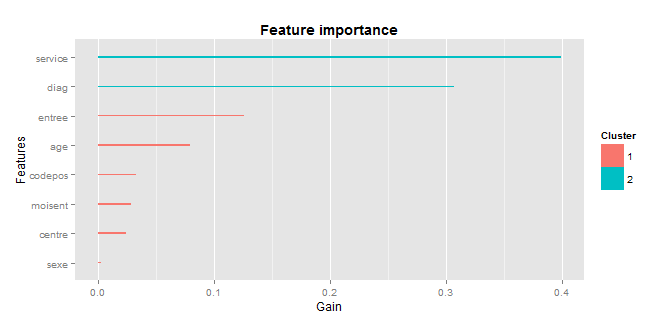
\includegraphics [width =12cm]{Sans_ID.png}
 \end{center}
 \end{figure}
\end{frame}

\begin{frame}[c]
\frametitle{Analyse des résultats}
 \begin {figure}[!ht]
 \caption{Analyse de l'importance des prédicteurs - Avec ID}
 \begin{center}
  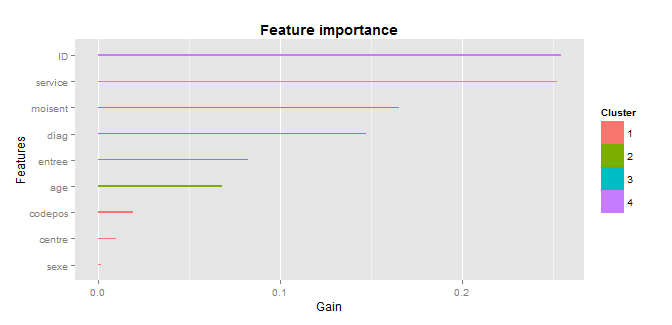
\includegraphics [width =12cm]{Avec_ID.png}
 \end{center}
 \end{figure}
\end{frame}

\begin{frame}[c]
\frametitle{}
\begin{center}
 {\Huge Fin}
\end{center}
\end{frame}

\end{document}

